\documentclass[11pt]{article}
\usepackage[margin=1.5in]{geometry}
\usepackage{fontspec}
\usepackage{xcolor}
\definecolor{darkblue}{rgb}{0,0,0.5}
\usepackage[colorlinks=true,allcolors=darkblue]{hyperref}
\usepackage{amsmath}
\usepackage{amssymb}
\usepackage{booktabs}
\usepackage{enumitem}
\setlist{noitemsep}
\usepackage{caption}
\usepackage{subcaption}
\usepackage{sidecap}
\sidecaptionvpos{figure}{c}
\usepackage{graphicx}
\graphicspath{{image/}}
\usepackage[sorting=ynt,style=authoryear,uniquename=false]{biblatex}
\addbibresource{paper.bib}
\usepackage{tikz-cd}
\usetikzlibrary{decorations.pathmorphing}
\DeclareMathOperator{\softmax}{softmax}
\DeclareMathOperator{\relu}{relu}

\title{Imaginary speech synthesis, part 1}
\author{%
  Kuan Yu \qquad Simon Untergasser \qquad Jörg Schwartz\\
  \textit{\{kuanyu, untergasser, jschwartz\}@uni-potsdam.de}\\
  \\
  Master's Program in \emph{Cognitive Systems}\\
  University of Potsdam}
\date{September 2018}

\begin{document}
\maketitle

% Number of words: 10k-12k
% Structure:
%     Title Page
%         Title + Abstract(~200w)
%     Intro
%         general -> topic specific -> your idea
%         highlight main contributions
%     Related Work
%         Who is also working in this area?
%         What is the current state?
%         What is the basis for your work? What is different to them?
%     Methods
%         Explain everything of your project (data, model,...)
%         If additional input is necessary to understand you project, maybe it is worth to give some space here?
%     Results and Discussion
%         Show your stats, explain your evaluation (metric)
%         discuss also things that did not work
%     Conclusion
%         Sum up your project (again) and highlight your main contributions (development and results)
%     Bib
%         pay attention to consistent citation structure
%         check whether your cites are correct

\begin{abstract}
  In this project we examine the application of complex-valued spectrograms
  in the domain of neural speech synthesis.
  In a text-to-speech task we train a modified transformer model to produce complex-valued spectrograms
  for audio clips from the transcribed character sequences.
  The outputs can then be transformed into waveforms directly via the inverse Fourier transform.
  We use a real-valued implementation for the complex-valued network,
  by treating the real and the imaginary parts of the complex numbers separately.
  However we also discuss the possibility for a network using complex calculus.

  Our attempt was not successful.
  The model failed to learn the alignment between the characters and the spectrogram frames.
  In this paper we explain our work,
  investigate the causes of failures,
  discuss the difficulties in speech synthesis and complex-valued modeling,
  and suggest possible remedies for a future research.
\end{abstract}

\section{Introduction}

In recent years audio synthesis has gathered a lot of attention.
While being also a traditionally very active field,
research shifted from concatenative synthesis to using neural models
for end-to-end generation.
Especially the subfield of synthesizing speech is of great interest
in applications such as text-to-speech (TTS) systems.
Early models used recorded pieces of speech and concatenated them to words,
and a step further went models which used single phonemes and interpolated between them
\parencite{taylor2009text}.
Although clear and intelligible the speech tends to sound emotionless and unnatural.
The uprise of artificial neural networks also gave rise to new ideas in speech synthesis.
End-to-end systems such as Char2Wav \parencite{sotelo2017char2wav},
Tacotron \parencite{wang2017tacotron}, and Deep Voice \parencite{arik2017deep}
have shown the effectiveness and simplicity of neural TTS (NTTS) models.
These systems take transcriptions namely sequences of characters as inputs,
and produce sequences of audio samples as outputs.

Directly predict audio samples faces the challenge of outputting sequences of considerable lengths.
For the highest quality audible by humans, a sample rate of 44.1 kHz,
namely 44\,100 steps of output per second of speech, is required.
Such systems must model complicated dependencies over a great number of time steps.
The sequential nature of these dependencies also demands a long computation time.
However using spectral analysis through short-time Fourier transform (STFT),
a large number of audio samples can be substantially reduced to a small number of spectrogram frames
without loss of information.
Some NTTS systems predict frames of magnitude spectrograms
and reconstruct the audio samples using a vocoder.
The reconstruction process is not a straightforward inversion of STFT (ISTFT),
since the phase information in the complex-valued spectra is not preserved in real-valued magnitude spectra.
The vocoder may use a pre-existing algorithm such as Griffin-Lim \parencite{griffin1984signal}
for estimating the phase information, or it may be another learned neural network.
The latter option is more computationally expensive,
but produces more natural-sounding speech \parencite{shen2018natural}.
We aim to develop an NTTS system which predicts the full complex-valued spectrograms,
thereby removing the necessity for a vocoder,
which can be replaced with a simple ISTFT component.
This was the main goal of our project.

Complex-valued networks are a rare but rewarding research topic \parencite{trabelsi2017deep}.
Due to the complex nature of spectral analysis,
speech modeling with complex calculus is the natural option
\parencite{hu2016initial, fu2017complex, nakashika2018complex}.
However, a complex number can be treated as a pair of real numbers,
and \textcite{drude2016appropriateness} argued that real-valued implementations
of complex-valued networks are just as effective.
We planned to eventually implement a model using complex calculus,
but due to various difficulties, this goal had to be postponed to the future.
In this project we experimented with models with real-valued features and outputs
from the real and imaginary parts of the complex-valued spectrogram frames.

Neural models for sequence-to-sequence learning has been developed and used in other tasks
such as statistical machine translation (SMT) \parencite{cho2014learning, sutskever2014sequence}.
The transformer is a more recent architecture developed for SMT with great success \parencite{vaswani2017attention}.
The architecture relies on attention layers,
as opposed to the conventional recurrent and convolutional layers.
It has since been used for constituency parsing \parencite{kitaev2018constituency},
language generation \parencite{liu2018generating},
image generation \parencite{parmar2018image},
and speech recognition \parencite{zhou2018syllable, zhou2018multilingual}.
Another goal of our project is to apply the transformer for speech synthesis.

Our attempt did not satisfy our goals.
However, we made effectual revisions to the transformer in our open source implementation.%
\footnote{\url{https://github.com/i-synth/i-synth}}
We would like to share what we have learned,
to discuss the causes of failures,
and to speculate possible remedies for a future research.

In this paper, we first describe the research background
and introduce the works which motivated our project (Section~\ref{sec:background}).
Then we explain our experiment setup, our model,
and the training process (Section~\ref{sec:methods}).
Finally we discuss the results and present our conclusion
(Section~\ref{sec:results}\&\ref{sec:conclusion})

\section{Background}\label{sec:background}

\subsection{NTTS systems}

\begin{figure}
  \centering
  \begin{tikzcd}
    T^{\ast}_{0} \ar[bend left]{r} \ar[bend right]{rr} \ar[bend left]{rrr} &T^{\ast}_{1} \ar[bend right]{r} \ar[bend left]{rr} &T^{\ast}_{2} \ar[bend left]{r} &T^{\ast}_{3}\\
  \end{tikzcd}
  \caption[]{\label{fig:autoreg}An autoregressive network.}
\end{figure}

Neural speech synthesis models generates target sequences \(T^{\ast}\),
which are constructed from the output space \(T\),
either audio samples or spectrogram frames.
They are commonly autoregressive networks
which constructs a target sequence one step at a time,
conditioning on the previous steps,
as shown in Figure~\ref{fig:autoreg}.
End-to-end NTTS models are sequence-to-sequence neural networks
consisting of an encoder and a decoder,
trained jointly with pairs of sequences.
The encoder learns a representation for the source sequences \(S^{\ast}\),
which are constructed from the transcript alphabet \(S\).
The decoder learns to predict the next step in the target sequence
conditioning on the encoded source sequence and previous target steps.
As a whole, it models the mapping
\(\forall i \in \mathbb{N}, \left(S^{\ast}, T^{\ast}_{0 \ldots i}\right) \to T^{\ast}_{i+1}\).
Since these sequences vary in their lengths,
a multi-layer perceptron (MLP) is not the ideal architecture.

Recurrent networks are suitable choices for speech generation.
One such example is SampleRNN \parencite{mehri2016samplernn},
a sample-level model consisting of a hierarchy of modules.
The final MLP module predicts individual samples,
while each previous recurrent module receives information over
an increasingly longer timescale with a lower temporal resolution.
This design shortens the distance of information flow from past steps.
Another option for effective sample-level modeling is to use
a convolutional network with hierarchical dilation to expand the receptive field,
which is the design behind WaveNet \parencite{van2016wavenet}.
Both models can be modified for speech synthesis by conditioning locally
on the content of speech, and possibly also globally on the style.

Char2Wav \parencite{sotelo2017char2wav} is a NTTS models using SampleRNN as the decoder,
and a bidirectional recurrent network as the encoder.
Similarly, Deep Voice \parencite{arik2017deep} uses a variant of WaveNet as the vocoder.
However the conditioning features for the vocoder are linguistic and acoustic information
produced by additional models,
including notably an recurrent encoder-decoder which converts texts to phonemes.
By contrast, Tacotron \parencite{wang2017tacotron} models speech
on the level of spectrogram frames,
with both linear and mel scales \parencite{stevens1937scale}.
The encoder is a CBHG network consisting of
a convolutional filter bank \parencite{qu2016learning} for learning ngram representations,
a highway network \parencite{srivastava2015highway} for extracting high-level features,
and a bidirectional recurrent network for incorporating more contextual information.
The decoder is a recurrent network predicting
multiple mel-scale magnitude frames at a time,
followed by a CBHG post-processing network
which converts the frames from mel scale to linear scale.
The linear magnitude spectrogram frames are converted to audio samples
using the Griffin-Lim algorithm.
In Tacotron 2 \parencite{shen2018natural},
the Griffin-Lim vocoder is replaced with a WaveNet model
using mel spectrograms as features.
Inspired by Tacotron,
Deep Voice 2 \parencite{arik2017deep2} adopts frame-level modeling.
On top of that, Deep Voice 3 \parencite{ping2017deep} has all recurrent layers
replaced with convolutional ones.

In all these NTTS systems except for the original Deep Voice,
attention-based recurrent or convolutional layers are used
for the decoder to condition on the encoder outputs.
Between the source steps and the target steps,
the dependency alignment is expected to be globally linear,
since the speech progresses according to the transcript.
Locally, however, the alignment is uncertain and may linger or skip forward.
Attention mechanisms are useful for detecting and aggregating these dependencies.

\subsection{Attention and transformer}

\subsubsection*{Attention mechanisms}

A general description for the commonly used soft attention is as follows,
given a query vector and multiple value vectors:

\begin{enumerate}
  \item The query determines a scalar weight for each value;
  \item The weights are then normalized to a probability distribution over the values, typically with
    the \(\softmax\)\footnote{\(\softmax : \mathbb{R}^{n} \to \mathbb{R}^{n},
      x_{i} \mapsto \exp x_{i} / \sum_{j=1}^{n}{\exp x_{j}}\)} function;
  \item The summary is simply the weighted sum of the values.
\end{enumerate}

\textcite{bahdanau2014neural} introduced an attention mechanism to SMT known as additive attention,
typically used in a recurrent structure.
The recurrent state is used as query.
Each value vector is concatenated with the query and passed into an MLP to produce the attention weight.
The usual choice for the MLP has a single hidden layer with \(\tanh\) activation.
\textcite{luong2015effective} introduced another mechanism where the attention weight is simply
the dot product between the query and the value.
This is known as dot-product or multiplicative attention.
\textcite{daniluk2017frustratingly} introduced key-value attention,
where the value vectors are split into two parts, the values and the keys.
Only the key vectors are used with the query to produce the weights.
This separates the tasks for the model to learn good representations for the values and the keys.

\begin{figure}
  \begin{subfigure}{0.5\textwidth}
    \centering
    \begin{tikzcd}
      &\hat{x}_{1} &\hat{x}_{2} &\hat{x}_{3}\\
      &\bullet{} \ar[violet]{u} &\bullet{} \ar[violet]{u} &\bullet{} \ar[violet]{u}\\
      &x_{0} \ar[red, bend left]{u} \ar[blue]{u} \ar[blue]{ur} \ar[blue]{urr} &x_{1} \ar[red, bend left]{u} \ar[blue]{u} \ar[blue]{ur} \ar[blue]{ul} &x_{2} \ar[red, bend left]{u} \ar[blue]{u} \ar[blue]{ul} \ar[blue]{ull}\\
    \end{tikzcd}
    \caption*{Encoder self-attention}
  \end{subfigure}%
  \begin{subfigure}{0.5\textwidth}
    \centering
    \begin{tikzcd}
      &\hat{x}_{1} &\hat{x}_{2} &\hat{x}_{3}\\
      &\bullet{} \ar[violet]{u} &\bullet{} \ar[violet]{u} &\bullet{} \ar[violet]{u}\\
      &x_{0} \ar[red, bend left]{u} \ar[blue]{u} \ar[blue]{ur} \ar[blue]{urr} &x_{1} \ar[red, bend left]{u} \ar[blue]{u} \ar[blue]{ur} &x_{2} \ar[red, bend left]{u} \ar[blue]{u}\\
    \end{tikzcd}
    \caption*{Decoder self-attention}
  \end{subfigure}
  \caption[]{\label{fig:layer}Self-attention layers.
    Arrows of the same color denotes linear transformations with the same parameters.
    The red arrows produce the queries,
    the blue arrows produce the values and keys,
    and the black bullets are the attention cells
    which produce the summaries.
    The purple arrows produce the outputs,
    which may be part of the next layer.}
\end{figure}

One common application of attention is for the decoder to attend to the encoder outputs,
but it can also be used for both the encoder and the decoder to attend to its own data
without any recurrent structure \parencite{parikh2016decomposable}.
This is known as self-attention or intra-attention.
In sequence learning, self-attention means that a query is simply one time step among the sequence,
and the values are the whole sequence or a subsequence.
The summarized value becomes an annotated representation for data at the time step queried,
with contextual knowledge of all data within the attended time steps.
Due to the autoregressive nature of the decoder,
it must not attend to the future steps.
Figure~\ref{fig:layer} illustrates the self-attention layers.

\begin{figure}
  \begin{subfigure}{0.5\textwidth}
    \centering
    \begin{tikzcd}
      &\hat{x}_{1} &\hat{x}_{2} &\hat{x}_{3}\\
      &+ \ar[violet]{u} &+ \ar[violet]{u} &+ \ar[violet]{u}\\
      \ar[red]{ur} &x_{0} \ar[blue]{u} \ar[red]{ur} &x_{1} \ar[blue]{u} \ar[red]{ur} &x_{2} \ar[blue]{u}\\
    \end{tikzcd}
    \caption*{Convolutional}
  \end{subfigure}%
  \begin{subfigure}{0.5\textwidth}
    \centering
    \begin{tikzcd}
      &\hat{x}_{1} &\hat{x}_{2} &\hat{x}_{3}\\
      \ar[red]{r} &\bullet{} \ar[violet]{u} \ar[red]{r} &\bullet{} \ar[violet]{u} \ar[red]{r} &\bullet{} \ar[violet]{u}\\
      &x_{0} \ar[blue]{u} &x_{1} \ar[blue]{u} &x_{2} \ar[blue]{u}\\
    \end{tikzcd}
    \caption*{Recurrent}
  \end{subfigure}
  \caption[]{\label{fig:conv-rec}A convolutional layer with filter size 2 and stride 1,
    and a recurrent layer where the black bullets denote the recurrent cell,
    cf. Figure~\ref{fig:layer}.}
\end{figure}

For comparison, Figure~\ref{fig:conv-rec} illustrates the more commonly used convolutional and recurrent layers
in the context of sequence learning.
In a convolution layer, each step can only access information from a fixed number of input steps,
but the computations for all input steps are independent and can be parallelized.
In a recurrent layer, the recurrent state carries information from all past steps,
but the sequential nature makes training slow.
The recurrent state may be an information bottleneck due to its fixed size,
and long distance dependencies may be difficult to learn.
While self-attention layers combine the advantages of convolutional layers and recurrent layers,
its computational complexity is quadratic instead of linear with respect to the length of the sequence,
since each step may query every other step.

Without either locality or temporal dependency,
the attention mechanism does not respect the ordering of a sequence.
\textcite{gehring2017convolutional} proposed to add positional information to the data,
in the form of a learned position embedding.
\textcite{vaswani2017attention} proposed to hard-code the positional information as sinusoids.
For dimension \(i\) and position \(j\), the encoding is defined as
\(p(j, 2i) = \sin \left( j / 10000^{2i/d} \right)\) and
\(p(j, 2i+1) = \cos \left( j / 10000^{2i/d} \right)\)
where \(d\) is the total number of dimensions.
The motivation is that the wavelengths form a geometric progression from \(\tau\) to \(10000 \tau\),
and that the relative distance between positions can be expressed as a linear function.
Unlike with a learned position embedding,
the length of sequences are not limited by the maximum position learned.
A similar encoding is used in Deep Voice 3.

\subsubsection*{Transformer}

The transformer uses scaled dot-product attention,
a novel variant of key-value dot-product attention.
The attention weights are divided by the square root of the representation dimension
before normalized by the \(\softmax\) function.
The scaling normalizes the variance of dot products.
On top of that, it introduced multi-head attention.
The query space is split into multiple disjoint subspaces.
Each split is an attention head.
The same is done for the key space and the value space.
For each head, the scaled dot-product attention produces a summary,
and the combined summary is their concatenation,
namely the direct sum of the subspaces.
Since each head decides its own list of attention weights,
the same position can be treated with different importance in different subspaces of its representation.
\textcite{vaswani2017attention} explained the splitting of heads
as projections to subspaces with learned linear transformations.
In order to simplify the interpretation,
we treat these linear transformations as procedures immediately before the attention mechanism,
and the projection maps are reduced to fixed orthogonal projections,
implemented as taking subvectors.

Since the attention mechanism alone merely produces a summary from a linear combination of values,
the transformer also uses position-wise MLPs to increase the depth.
Each MLP consists of two layers with
\(\relu\)\footnote{\(\relu : \mathbb{R} \to \mathbb{R}, x \mapsto \max(0, x)\)} activation between,
applied to each position separately.
Each attention layer or MLP is followed by dropout \parencite{srivastava2014dropout},
residual connection \parencite{he2016deep}, and layer normalization \parencite{ba2016layer}.
They are the sublayers in a transformer layer.
A transformer layer in the encoder consists of a self-attention layer followed by an MLP,
and a decoder layer has a secondary attention layer attending to the encoder outputs
in order to condition the construction of target sequences on the source sequences.
Figure~\ref{fig:transformer} illustrates the full architecture.

\begin{SCfigure}[4]
  \centering
  \tikz[overlay]{
    \draw[green] (0.0,-1.25) rectangle (1.0,0.75);
    \draw[green] (2.2,-1.25) rectangle (3.2,1.9);}
  \begin{tikzcd}[column sep=tiny]
    &&\hat{T}^{*}_{1 \ldots i+1}\\
    &&\cdot \ar[violet]{u}\\
    \cdot \ar[blue]{rr} &&\bullet{} \ar[violet, rightsquigarrow]{u}\\
    \bullet{} \ar[violet, rightsquigarrow]{u} &&\bullet{} \ar[red]{u}\\
    + \ar[blue, bend left]{u} \ar[red, bend right]{u} &&+ \ar[blue, bend left]{u} \ar[red, bend right]{u}\\
    S^{*} \ar[violet]{u} &P \ar[dashed]{ul} \ar[dashed]{ur} & T^{*}_{0 \ldots i} \ar[violet]{u}\\
  \end{tikzcd}
  \caption[]{\label{fig:transformer}A transformer
    with the encoder on the left and the decoder on the right.
    \(P\) is the position encoding.\\
    The straight arrows are linear transformations,
    the dashed arrows are identity functions,
    and the squiggly arrows are position-wise MLPs.\\
    The coloring matches the scheme in Figure~\ref{fig:layer}.
    The same color signifies the same interpretation,
    and not (necessarily) the same parameters.\\
    The green boxes mark the transformer layers,
    which can be stacked to increase the depth.\\
    The graph omits the residual connections and layer normalizations after each sublayer.}
\end{SCfigure}

\subsection{Complex-valued networks}

One of the motivations for this project was to investigate the dynamics of complex numbers
and the application of complex calculus in neural networks for speech synthesis.
However due to various difficulties, this promise was never fulfilled.
Nevertheless we would like to discuss our research on this issue for future references.
The reader may feel free to skip this section.

In the following we discuss the implementation details behind complex-valued neural networks,
in particular the appropriate activation function, mostly thanks to the work of \textcite{scardapane2018complex}.

We represent a complex number $z$ in the set of complex numbers $\mathbb  C$ as $z=a+ib$, where $a=\text{Re}(z)$ and $b=\text{Im}(z)$, with $a, b\in \mathbb R$, denote, respectively,  the real and the imaginary part of $z$, and $i=\sqrt{-1}$. %For simplicity, we also use $z_R$ and $z_I$ to denote real and imaginary parts of $z$.
Magnitude and phase are given by $|z|$ and $\phi(z)$, and $z^*=a-ib$ denotes the \textit{complex conjugate} of $z$.
% The Hermitian transpose of a vector or matrix is given by $(\cdot)^ H$ and the transpose is denoted as $(\cdot)^\top$.

Any complex-valued function $f\colon \mathbb C\to\mathbb C$ on the complex domain can be written as a sum of two bi-variate real-valued functions $u(\cdot, \cdot), v(\cdot,\cdot)\colon \mathbb R\times\mathbb R\to \mathbb R$ via
\begin{equation}
f(z) = u(a, b) + iv(a,b), \quad z=a+ib\in \mathbb C.
\end{equation}
Then $f$ is said to be \textit{real-differentiable}, if the partial derivatives $\partial u$ and $\partial v$ with respect to $a, b\in\mathbb R$ exist. If the partial derivatives of $f$ also satisfy the $\textit{Cauchy-Riemann}$ equation
\begin{equation}
\frac{\partial u(a,b)}{\partial a} = \frac{\partial v(a,b)}{\partial b}\text{  and  }\frac{\partial v(a,b)}{\partial a} = - \frac{\partial u(a,b)}{\partial b},
\end{equation}
then $f$ is said to be \textit{analytic} or \textit{holomorphic} with respect to $a,b\in \mathbb R$. Note that, if $f$ is real-valued (and hence $v(a,b)=0$), the aforementioned condition for $f$ to be holomorphic reduces to
\begin{equation}
\frac{\partial u(a,b)}{\partial a}=-\frac{\partial u(a,b)}{\partial b} = 0.
\end{equation}
For the \textit{standard} complex derivative of a complex-valued function $f$ to exist in a meaningful way in the complex variable $z\in \mathbb C$, we have to ensure that, independent for every path $\Delta z\to 0$ in the complex plain, the limes
\begin{equation}
f^\prime(z)  = \frac{\text d f}{\text d z}= \lim_{\Delta z\to 0} \frac{f(z+\Delta z) - f(z)}{\Delta z}
\end{equation}
exists.
Note that the Cauchy-Riemann equations stated above summarize the conditions for the derivative to assume the same value regardless of the direction of approach when $\Delta z\to 0$. An example that this does not hold for simple (real-differential) functions in the complex domain is given by the conjugate function $f(z) = z^*$, which yields two different paths:
\begin{equation}
\lim_{\eta\to 0}\frac{(z+\eta)^*- z^*}{\eta}=1,\quad\lim_{i\eta\to 0}\frac{(z+ i\eta)^* - z^*}{i\eta} = -1, \quad \eta\in \mathbb R.
\end{equation}
Particularly, the following conditions are equivalent statements about a complex function $f$:
\begin{enumerate}
\item The derivative $f^\prime(z)$ exists and is continuous.
\item The function $f$(z) is holomorphic (i.e. analytic in  $z$).
\item $f$ satisfies the Cauchy-Riemann conditions in $z$.
\item All derivatives of $f(z)$ exist and $f$ has a convergent power series in $z$.
\end{enumerate}
Furthermore, it is a simple consequence of the Cauchy-Riemann conditions that
$$f(z) = u(a,b) + iv(a,b)$$
is holomorphic only if the functions $u(a,b)$ and $v(x,y)$ both satisfy the \textit{Laplace's equation} given by
$$\frac{\partial^2 u(a,b)}{\partial x^2} + \frac{\partial^2 u(a,b)}{\partial y^2} = 0 \quad\text{and}\quad\frac{\partial^2 v(a,b)}{\partial x^2} + \frac{\partial^2 v(a,b)}{\partial y^2} = 0 .$$
Such functions are also known as \textit{harmonic} functions. Thus if either $u(a,b)$ or $v(a,b)$ fail to be harmonic, the function $f(z)$ can not be complex differentiable.

In summary, the simple hypothesis that $f^\prime(z)$ exists, imposes a firm structure on both $u(a,b)$ and $v(a,b)$, the real and imaginary parts of the functions (and consequently on $f(z) = f(a,b)$), which is stronger than the mere existence of the partial derivatives.

Although many important functions are holomorphic, including $z^n$, $\exp(z)$, $\ln(z)$, $\sin(z)$ and $\cos(z)$ and hence differentiable in the standard complex sense, various  commonly encountered useful functions are not:
\begin{enumerate}
\item The functions $f(z)=\text{Re}(z) = \frac{z+z^*}{2} = a$ and $g(z) = \text{Im}(z)=\frac{z-z^*}{2i}=b$ fail the Cauchy-Riemann conditions.
\item The function $f(z) = |z|^* = z^*z = a^* + b^*$ is not harmonic.
\item Any \textit{nonconstant purely real-valued} function f(z) (for which it must be the case that $v(a,b)=0$) failes the Cauchy-Riemann condition. In particular the real function $f(z) = |z| = \sqrt{z^* z} = \sqrt{a^2 + b^2}$ is not differentiable.
\end{enumerate}
Thus we have the classic result that the only holomorphic real-valued functions are the constant real-valued functions. If a gradient procedure for determining the optimum is desired, we are immediately stymied by the fact that the purely real non-constant squared-error loss functional is not analytic and therefore its derivative does not exist in the conventional sense of a complex derivative (which applies only to holomorphic functions).

Most cost functions used in practice for artificial neural networks do not satisfy the Cauchy-Riemann condition due to their  real-valued output and hence are not complex differentiable. Furthermore, \textsc{Liouville's theorem} states that \textit{any bounded function that is also holomorphic, must be a constant}; conversely, if the function is bounded, but not a constant, it can not be holomorphic. Due to the preference for bounded activation functions before the introduction of the ReLU, many authors preferred bounded functions to holomorphic ones. It is worth mentioning however that holomorphic functions can be leveraged for computational efficiency purposes. Using complex differentiable functions allows one to share gradient values, since the activation satisfies the Cauchy-Riemann equations and thus the computation of only 2 instead of 4 different gradients are required during back-propagation.

An elegant approach which allows one to handle non-holomorphic functions directly in the complex domain (instead of the need of switching back and forth between the complex domain and the gradients computation in the real domain) is due to Wirtinger, which relaxes the strong requirement for differentiability and defines a  less stringent form for the complex domain. \textit{Wirtinger Calculus} or $\mathbb C\mathbb R$\textit{-Calculus} describes how this new theoretical framework can be used for defining complex differential operators that allow computation of derivatives in a very straightforward manner in the complex domain, thus extending the standard partial derivative to non-holomorphic functions, that are nonetheless real-differentiable. We will call this the $\textit{real-derivative}$  or $\mathbb R\textit{-derivative}$ of a possible non-holomorphic function in order to avoid confusion with the standard complex derivative, or $\mathbb C\textit{-derivative}$ of a holomorphic function (this extension, when applied to holomorphic functions, reduces the real-derivative to the standard complex derivative).

The main idea is to consider $f$ as a function of both $z$ and its complex conjugate $z^*$. Doing so will allow us to view any real-differential function $f$ as holomorphic in $z$, if we keep $z^* $ constant, respectively holomorphic in $z^*$ if we keep $z$  constant. Note that the non-holomorphic (non-analytic in $z$) functions given as examples above can  all be written in the form $f(z, z^*)$, where they \textit{are} holomorphic in $z=a+ib$ \textit{for fixed} $z^*$ and holomorphic in $z^*= a-ib$ \textit{for fixed} $z$ (that is, if we make the substitution $w=z^*$, they are analytic in $w$ for fixed $z$). Upon substituting
\begin{equation}
a = \frac{z+z^*}{2}, \quad b=\frac{z-z^*}{2i},
\end{equation}
it can be shown that this fact is true in general for any complex- or real-valued function
$$f(z) =f(z, z^*) = f(a,b) = u(a,b) + iv(a,b)$$
of a complex variable for which the real-valued functions $u$ and $v$ are differentiable as functions of the real variables $x$ and $y$, i.e. the mapping $f$ can be rewritten as a bi-variate function of both $z$ and $z^*$. In essence, the so-called \textit{conjugate coordinates,}
\begin{equation}
c \triangleq (z, z^*)^\top\in\mathbb C\times \mathbb C, z=a+ib\text{   and  } z^*= a-ib
\end{equation}
can serve as a formal substitute for the real  $r\triangleq (x,y)^\top$ representation of the point $z=x+iy\in \mathbb C$.

If $f$ is real-differentiable, i.e., $u(a,b)$ and $v(a,b)$ are differentiable with respect to the real-valued variables $a$ and $b$, we can compute $(\partial f/\partial z)$ and $(\partial f/\partial z^*)$ by treating $z$ and $z^*$ as two independent variables, thus considering $z$ (respectively $z^*$) as a constant. For a general complex- or real-valued function $f(c)=f(z,z^*)$ consider the pair of partial derivatives of $f(c)$ called \textit{Wirtinger operators} formally (since one cannot truly vary $z=a+ib$ while keeping $z^*=a-ib$ constant) defined by

\begin{equation}
\begin{split}
\mathbb R\text{-derivative of } f(c) &\triangleq \frac{\partial f(z, z^*)}{\partial z}\mid_{z^* = \text{const.}},\\%=\frac{\partial f}{\partial z}  = \frac{1}{2}\Big(\frac{\partial f}{\partial a} - i\frac{\partial f}{\partial b}\Big),\\
\mathbb R^*\text{-derivative of } f(c)&\triangleq \frac{\partial f(z, z^*)}{\partial z^*}\mid_{z = \text{const.}},%=\frac{\partial f}{\partial z^*}  = \frac{1}{2}\Big(\frac{\partial f}{\partial a} + i\frac{\partial f}{\partial b}\Big)
\end{split}
\end{equation}
where the formal partial derivatives are viewed as standard complex partial derivatives ($\mathbb C$-derivatives) taken with respect to $z$ in the first case and with resepct to $z^*$ in the second. For example, with $f(z, z^*) = z^2 z^*$ we have
$$ \frac{\partial f}{\partial z} = 2zz^*\text{  and   }\frac{\partial f}{\partial z^*} = z^2.$$
It can be shown that the $\mathbb R$-derivative and $\mathbb R^*$-derivative formally defined above are equivalent to the expression
\begin{equation}
\begin{split}
\mathbb R\text{-derivative of } f(c) &=\frac{\partial f}{\partial z}  = \frac{1}{2}\Big(\frac{\partial f}{\partial a} - i\frac{\partial f}{\partial b}\Big),\\
\mathbb R^*\text{-derivative of } f(c)& =\frac{\partial f}{\partial z^*}  = \frac{1}{2}\Big(\frac{\partial f}{\partial a} + i\frac{\partial f}{\partial b}\Big),
\end{split}
\end{equation}
where the partial derivatives with respect to $a$ an $b$ are \textit{true} (i.e., non-formal) partial derivatives of the function $f(z) = f(a,b)$, which is always assumed in this note to be differentiable with respect to $a$ and $b$ (i.e., to be $\mathbb R$-differentiable). Thus, it is the right-hand-sides of the expression in $(9)$ which make the formal definition rigorous. Note that from the above equality, we immediately have the properties
$$\frac{\partial z}{\partial z}=\frac{\partial z^*}{\partial z^*} = 1\quad\text{ and  } \quad\frac{\partial z}{\partial z^*}=\frac{\partial z^*}{\partial z}=0.$$
Additionally, the following properties hold:
\begin{enumerate}
\item The condition $\frac{\partial f}{\partial z^*} = 0$ is true for an $\mathbb R$-differentiable function $f$ if and only if the Cauchy-Riemann conditions are satisfied. Thus a function $f$  is holomorphic if and only if it does not depend on the complex conjugated variable $z^*$, i.e., when $f(z, z^*) = f(z)$.
\item The $\mathbb R$-derivative, $\frac{\partial f}{\partial z}$, of an $\mathbb R$-differentiable function $f$ is equal to the standard $\mathbb C$-derivative, $f^\prime(z)$, when $f(z, z^*)$ is independent of $z^*$, i.e., when $f(z, z^*) = f(z)$.
\item An $\mathbb R$-differentiable function $f$ is holomorphic in $z^*$ if and only if it does not depend on the variable $z$, i.e., when $f(z, z^*) = f(z^*)$, which is true if and only if $\frac{\partial f}{\partial z} = 0$.
\end{enumerate}
To summarize, an $\mathbb R$-differentiable function $f$ is holomorphic if and only if $\frac{\partial f}{\partial z^*} = 0$. We call this single condition the \textit{Cauchy-Riemann condition} for $f$ to be holomoprhic.

The $\mathbb R$-derivative and $\mathbb R^*$-derivative are both \textit{linear operators} which obey the \textit{product rule} of differentation. Furthermore, the following useful properties hold:
\begin{equation*}
\begin{split}
\frac{\partial f^*}{\partial z^* } &=\Bigg( \frac{\partial f}{\partial z}\Bigg)^*\\
\frac{\partial f^*}{\partial z } &=\Bigg( \frac{\partial f}{\partial z^*}\Bigg)^*\\
df &= \frac{\partial f}{\partial z} dz + \frac{\partial f}{\partial z^*}dz^*\quad \text{Differential Rule}\\
\frac{\partial h(g)}{\partial z} &= \frac{\partial h}{\partial g}\frac{\partial g}{\partial z} + \frac{\partial h}{\partial g^*}
\frac{\partial g^*}{\partial z}\quad \text{Chain Rule}\\
\frac{\partial h(g)}{\partial z^*} &= \frac{\partial h}{\partial g}\frac{\partial g}{\partial z^*} + \frac{\partial h}{\partial g^*}
\frac{\partial g^*}{\partial z^*}\quad \text{Chain Rule}.
\end{split}
\end{equation*}
A simple consequence of the above is that if $f$ is real-valued, i.e., $v(a,b)=0$, then $f(z)^* = f(z)$, so that we have the additional important identity that
\begin{equation}
f(z)\in\mathbb R\Rightarrow \Big(\frac{\partial f}{\partial z}\Big)^* = \frac{\partial f}{\partial z^*}.
\end{equation}
As a simple first application of the above, consider the problem of minimizing the real-valued squarer-error loss functional
$$\ell(z) = \text{E}(|\eta_k-z^*\xi_k|^2) = \text{E}((\eta_k-z^*\xi_k)^*(\eta_k-z^*\xi_k))\triangleq\text{E}(e^*_ke_k)$$
of complex random variables  $\xi_k$ and $\eta_k$ and unknown complex constant $z = a +ib$. Then the $\mathbb R^*$-derivative of $\ell(z)$ can be easily computed from the properties above to be
$$\frac{\partial \ell(z)}{\partial z^*} = \frac{\partial }{\partial z^*}\text{E}(e^*_ke_k) = \text{E}\Bigg(\frac{\partial e^*_k}{\partial z^*}e_k + e^*_k\frac{\partial e_k}{\partial z^*}\Bigg) = \text{E}(0\cdot e_k - e^*_k\xi_k) = -\text{E}(\xi_k e^*_k).$$
Similarly, it can be shown that the $\mathbb R$-derivative of $\ell(z)$ is given by
$$\frac{\partial \ell(z)}{\partial z} = -\text{E}(\xi^*_k e_k).$$
It is useful to view such a  pair of formal partial derivatives for a possibly non-holomorphic function as the natural generalization of the single complex derivative ($\mathbb C$-derivative) of a holomorphic function.

The main result in this context can be stated as follows:
Let $f\colon \mathbb R\times\mathbb R\to \mathbb C$ be a function of real variables $a$ and $b$ such that $g(z, z^*) = f(a,b)$, where $z = a + ib$ and $g$ is holomorphic with respect to $z^*$ and $z$ independently. Then the following properties hold:
\begin{enumerate}
\item The partial derivatives $$\frac{\partial g}{\partial z}= \frac{1}{2}\Big(\frac{\partial f}{\partial a} - i\frac{\partial f}{\partial b}\Big),\quad \frac{\partial g}{\partial z^*}= \frac{1}{2}\Big(\frac{\partial f}{\partial a} + i\frac{\partial f}{\partial b}\Big),$$can be computed by treating $z^*$ as a constant in $g$ (and $z$, respectively).
\item A necessary and sufficient condition for $f$ to have a stationary point is that $\partial g/\partial z=0$. Similarly, $\partial g/\partial z^*=0$ is also a necessary and sufficient condition
\end{enumerate}

Therefore, when evaluating the gradient, we can directly compute the derivatives with respect to the complex argument, rather than calculating individual real-valued gradients. The requirement for the analyticity of $g(z,z^*)$ with respect to $z$ an $z^*$ is independently equivalent to the condition of the real differentiability of $f(a,b)$ since we can move from one form to the function to the other using the simple linear transformation given above. When $f(z)$ is complex analytic, that is, when the Cauchy-Riemann conditions hold, $g(\cdot)$ becomes a function of only $z$, and the derivatives given by the statement above and the standard one coincide.

The difficulties that arise in complex-valued processing are mainly due to the selection of a suitable activation functions for the use in the optimization procedure for driving the weight update rule. The first issue is due to the conflict between boundedness and differentiabity of functions in the complex domain: because of \textsc{Liouville's theorem}, choosing a suitable activation function is more challenging than in the real case, as one has to choose between boundedness and analyticity. For example, the sigmoid non-linearity, which has been the typically used activation function for a real-valued multilayer perceptron, has periodic singular points. Since almost all activation function were bounded before the introduction of the ReLU, the initial approach to design CVNNs preferred non-analytic functions in order to preserve boundedness. In most cases, this was achieved by applying  real-valued activation functions $g_\mathbb R(\cdot)$ separately to the real and imaginary parts of a complex-valued input $z$
\begin{equation}
g(z) = g_\mathbb R(\text{Re}(z))+ i g_\mathbb R(\text{Im}(z)),
\end{equation}
which is also called a \textit{split activation function} \cite{}.

Another approach has been to to define joint-nonlinear complex activation functions, also named \textit{phase-amplitude} (PA) functions,
\begin{equation}
\begin{split}
g(z) &= \frac{z}{c+|z|/r},\\
g(z) &= \tanh \Big(\frac{|z|}{m}\Big)\exp(i\phi(z)),
\end{split}
\end{equation}
where $\phi(z)$ is the phase and $c, m$ and $r$ denote some positive constant. PA functions can be seen as the natural generalization of real-valued squashing functions such as the sigmoid.
% These functions cannot utilize the phase information effectively, as shown in .

It is also possible to use fully-complex activation functions that are analytic and bounded almost everywhere, such as in
\begin{equation}
g(z) = \tanh(z) = \frac{\exp(z)-\exp(-z)}{\exp(z) + \exp(-z)},
\end{equation}
which is the complex-valued extension of the hyperbolic tangent possessing periodic singular points at the imaginary points $i(0.5 + n)\pi$ with $n\in\mathbb N$. Doing so requires careful scaling of the inputs and initial weights to avoid these singularities during training.

Several extensions of the real-valued ReLU function have been proposed. However, its success in deep learning does not immediately translate to the complex-valued case, where using it in a split activation function results in poor performance  \cite{}. Due to this, \cite{} proposes modReLU, which is defined as
\begin{equation}
\text{modReLU}(z) = \text{ReLU}(|z| + b)\exp(i\phi(z)),
\end{equation}
where $z\in \mathbb C$ and $b$ is a learnable parameter. The intuition behind the design of the modReLU is to preserve the pre-activated phase $\phi(z)$, as altering it with an activation function severely impacts the complex-valued representation. modReLU does not satisfy the Cauchy-Riemann equations, and thus is not holomorphic.

We denote the complex activation that applies separate ReLUs on both the real and imaginary part with
\begin{equation}
\mathbb C\text{ReLU}(z) = \text{ReLU}(\text{Re}(z)) + i\text{ReLU}(\text{Im}(z)).
\end{equation}
$\mathbb C$ReLU satisfies the Cauchy-Riemann equations when both real and imaginary parts are the same time either strictly positive or strictly negative, i.e. when $\phi(z)\in (0, \pi/2)$ or $\phi(z)\in (\pi, 3\pi/2)$.

\section{Methods}\label{sec:methods}

\subsection{Experiment setup}

\subsubsection*{Dataset}

We used the LJ Speech Dataset for our project.%
\footnote{\url{https://keithito.com/LJ-Speech-Dataset/}}
This dataset consists of 13,100 audio clips each ranging in length between 1.11 and 10.10 seconds. It is a single speaker reading passages from 7 non-fictional books written between 1884 and 1964. With every clip comes a transcript. The data is nearly 24 hours of speech with over 225,000 words spoken. Table \ref{t:dataset} shows the relevant information of the data set.
\begin{table}
\centering
\begin{tabular}{ll}
  Total Clips & 13,100\\
  Total Words & 225,715 \\
  Total Characters & 1,308,678\\
  Total Duration & 23:55:17\\
  Mean Clip Duration  & 6.57 sec\\
  Min Clip Duration &	1.11 sec\\
  Max Clip Duration &	10.10 sec\\
  Mean Words per Clip & 17.23\\
  Distinct Words & 13,821\\
\end{tabular}
\caption{Statistics of the LJ Speech Dataset}
\label{t:dataset}
\end{table}

The clips were segmented automatically based on silence. Therefore the segmenting is not perfect. Most of the time on clip contains one sentence but that is not necessarily always the case. The transcripts was also automatically matched to the audio and later manually checked if the transcript fits the spoken text.
The audio clips are single-channel 16 bit WAV files with a sampling rate of 22,050 Hz. The transcripts come as csv-files with one record per line. Provided is an ID (the name of the file) the standard transcript and a normalized transcript. In the normalized transcription numbers, ordinals and monetary units are written in full words. \\

\subsubsection*{Data preprocessing}

We further processed the data in the following ways. In the transcription we found an inconsistent use of quotes and brackets. Furthermore it contained non-ascii characters. We cleaned all the transcripts of these flaws and lowercased them. To reduce computational complexity we downsampled the audio clips from 22,050 Hz to 8,000 Hz. Figure \ref{fig:downsampled} shows the spectogram of an example audio clip and its downsampled version.
\begin{figure}
  \begin{subfigure}{0.5\textwidth}
    \centering
        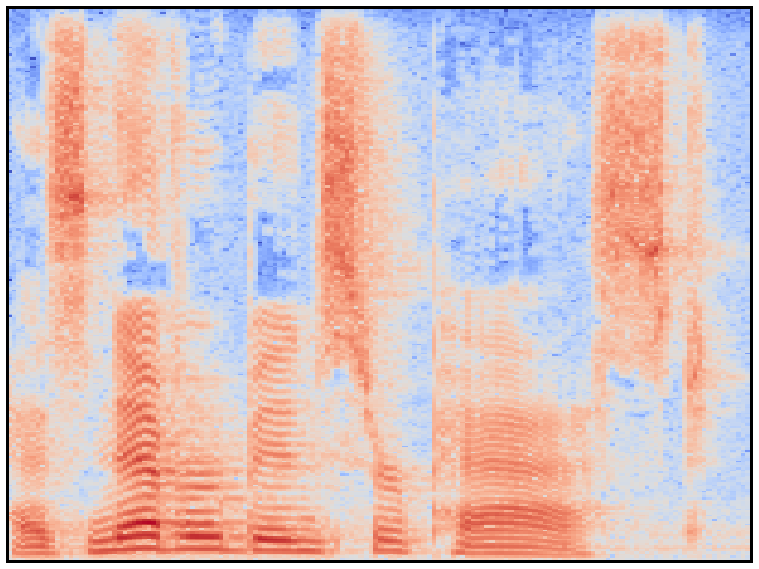
\includegraphics[width=0.9\textwidth]{image/original.pdf}
    \caption{22,050 Hz}
  \end{subfigure}%
  \begin{subfigure}{0.5\textwidth}
    \centering
    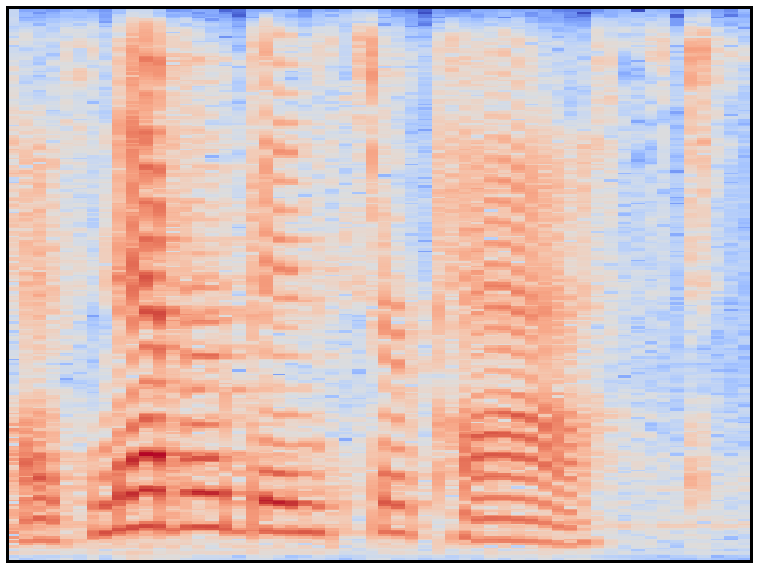
\includegraphics[width=0.9\textwidth]{image/downsampled.pdf}
    \caption{8,000 Hz}
  \end{subfigure}
  \caption{The spectogram of an example audio clip. (a) shows the original audio with 22,050 Hz sampling rate and (b) the downsampled to 8,000 Hz version.}{\label{fig:downsampled}}
\end{figure}
As one can clearly see, the overall resolution has decreased a lot. The information in the lower frequencies is preserved and higher frequencies are cut off. But since the most relevant frequencies for intelligibility lie in the range up to 4,000 Hz this would only affect the overall sharpness and brightness of the audio clips. They are still very good in quality but sound more muffled.

As is common in speech processing we transformed the data from the time domain to the frequency domain using STFT, for which we used the librosa package.%
\footnote{\url{https://librosa.github.io/}}
We conducted experiments with window sizes ranging from 128 to 8192 samples. In these ranges we tested hop sizes from half the window size to the full window size. We also tested different window functions ranging from the simple Boxcar over Blackman-Harris, Hamming and Hanning. For all these experiments we transformed a few audio clips and transformed them back via ISTFT.\@ The results of these experiments indicate, that the window size and also the hop size is uncritical because ISTFT can recreate the original signal perfectly. We then introduced some noise in the transformed data. We tried a convertion into mel scale, which reduces information. We also just reduced resolution of the data in the frequency domain. Then we performed ISTFT, now finding a result reduced in quality. The reduction of resolution clearly destroys some information, so that the reconstructed audio clip sounds unnatural. We found that the Boxcar window introduced stuttering and bursts of very high frequencies. Also too short windows introduced distortions.
Eventually we decided to to use a frame size of 512 samples and a hop size of 256 samples. To reduce spectral bleeding and the high frequency bursts we decided to use the very common Hanning window.
The longest audio clip in the data yielded 318 spectrogram frames.

Most models now preprocess the data further by calculating the power spectra of the frames. This is mostly due to the general assumption, that phase information is not important for speech processing. For speech recognition this seems to be true. But for speech generation phase information seems to be necessary. Most recent work introduces this information by learning another stage in the model which predicts the waveform, including phase information, from the power spectrum.
Since we are particularly interested in predicting a complex spectrum to get rid of this additional step, we don't convert the complex spectrum to the power spectrum.

\subsubsection*{Model overview and evaluation}%
\label{ssec:evaluation}

After STFT, each audio clip becomes a complex-valued spectrogram of height 257 and a variable width.
We discarded the highest frequency bin for simplicity,
and replaced it with zeros for ISTFT,
which had no noticeable effect on the quality of the restored audio.
Each spectrogram is regarded as a sequence of 256-dimensional frame vectors, of length \(t\).
The corresponding transcript is regarded as a sequence of characters, of length \(s\).
The characters are embedded in a 512-dimensional vector space.
The whole model can be viewed as a mapping \(\mathbb{R}^{s,512} \to \mathbb{C}^{t,256}\).
Since we only experimented with real-valued networks,
each complex number was treated as a pair of real numbers,
and the model was treated as \(\mathbb{R}^{s,512} \to \mathbb{R}^{t,512}\).

We randomly split the data into two parts for training and validation.
Most TTS models are evaluated manually by the mean opinion score,
often through crowdsourcing,
which was not feasible for our project.
In our experiments,
we mainly judge the model by the absolute error of the reconstructed linear spectrograms on the validation set,
and secondarily inspected the reconstructed spectrograms and audios.

\subsection{Network architecture}\label{sec:architecture}

We started with a faithful reimplementation of the original transformer,
but made various changes to the design during our experiments.
In order to explain our design choices,
here is an reexamination for the attention mechanisms.

\subsubsection*{Attention reexamined}

\begin{figure}
  \begin{subfigure}{0.5\textwidth}
    \centering
    \begin{tikzcd}
      v &&\\
      wt \cdot t \ar[violet]{u}{vw} &t \ar[swap]{l}{\softmax}\\
      vt \ar[blue]{u}{wv} \ar[blue, swap]{r}{kv} &kt + k \ar[rightsquigarrow, swap]{u}{\textrm{MLP}} &q \ar[red]{l}{kq}\\
    \end{tikzcd}
    \caption*{Additive attention}
  \end{subfigure}%
  \begin{subfigure}{0.5\textwidth}
    \centering
    \begin{tikzcd}
      v &&\\
      wt \cdot t \ar[violet]{u}{vw} &&\\
      vt \ar[blue]{u}{wv} \ar[blue, swap]{r}{kv} &kt \cdot^{T} k \ar[swap]{ul}{\softmax} &q \ar[red]{l}{kq}\\
    \end{tikzcd}
    \caption*{Dot-product attention}
  \end{subfigure}
  \caption[]{\label{fig:attention}Attention mechanisms with
    \(t\) time steps, \(q\) query dimensions, \(k\) key dimensions,
    \(v\) value dimensions, and \(w\) intermediate value dimensions.
    For the simplicity of notation,
    we use the shape of an object to denote the object itself.
    To unify matrix multiplication and batched dot product,
    we treated vectors as column matrices,
    and define \(A \cdot B := A B\)
    whereas \(A \cdot^{T} B := A^{T} B\).}
\end{figure}

Figure~\ref{fig:attention} demonstrates the general forms of additive attention and dot-product attention.
Given a query vector of \(q\) dimensions,
and a sequence of value vectors of \(v\) dimensions and \(t\) time steps,
packed into a value matrix of shape \(vt\),
the attention mechanism produces a summarized value vector of \(v\) dimensions.
Two matrices \(kq\) and \(kv\) performs the linear transformations
from the query space and the value space to the key space,
where the query and values can be matched to produce the attention weights.
Another linear transformation \(wv\) produces the actual values to be weighted.
Finally \(vw\) transforms the summary to a value vector for the next layer.
This process is repeated for each time step.
The interpretation of these linear transformations may vary in specific designs.
For example, with additive attention,
the key transformation \(kv\) is in fact part of the MLP after concatenation,
and the value transformation \(wv\) is usually the identity function,
unless key-value attention is used, in which case it is an orthogonal projection.
Also the final transformation \(vw\) may be part of the next layer.

Additive attention is computationally expensive.
The MLP has to operate on \(kt + k\) for all time steps,
which is a tensor with a shape of batch size times \(kt^{2}\) during training.
In dot-product attention, that tensor is immediately contracted.
Unless we restrict \(k\) to a very small number,
it is not feasible to apply additive attention in a fully attention-based model.
We experimented with \(k = 2, 4, 8, 16\) and found training to be much more difficult than
models with dot-product attention using a similar amount of memory.
The model learned slower per training step and each training step takes much longer.
Therefore we focused our experiments on dot-product attention.

\subsubsection*{Revisions}

\begin{figure}
  \centering
  \begin{tikzcd}
    v &&\\
    vt \cdot t \ar[violet, rightsquigarrow, swap]{u}{\textrm{MLP}} &&\\
    vt \ar[blue, dashed]{u} \ar[blue, dashed]{r} &vt \cdot^{T} v \ar[swap]{ul}{\softmax} &q \ar[red, rightsquigarrow, swap]{l}{\textrm{MLP}}\\
  \end{tikzcd}
  \caption{\label{fig:revis}Revised attention cell, cf. Figure~\ref{fig:attention}.}
\end{figure}

The linear transformation for keys and values are useful
if we wish to set the dimensions \(k\) and \(w\) to be different from \(v\).
However in the our transformer and the original,
all dimensions (\(q\), \(k\), \(v\), and \(w\)) are kept the same.
We observed that in dot-product attention,
the key transformation \(kv\) is in fact redundant.
By replacing \(kq\) with \(kv \cdot^{T} kq\) and \(kv\) with identity,
the resulting attention weights would remain the same.
Hence the model could simply learn the key transformation, if it is necessary at all,
as part of the query transformation.
Similarly, the value transformation \(wv\) is also redundant.
The model could simply learn \(vw\) as \(vw \cdot wv\),
due to the associativity of linear transformations.

Since the dot product is a bilinear form,
and both the key and the query transformations are linear,
the original dot-product attention can only model bilinear maps,
whereas the additive attention uses an MLP which is
a universal function approximator \parencite{hornik1989multilayer}.
\textcite{vaswani2017attention} observed that additive attention outperforms dot-product attention
for large representation dimensions while for small dimensions they perform similarly,
which motivated the proposed scaling factor.
We used an MLP for the query transformation.
While the attention weights are still linear with the value space,
the resulting summary is no longer a simple linear combination of values.
This is important for the self-attention layers,
where the query comes from the same space as the values.

Figure~\ref{fig:revis} illustrates our revised dot-product attention.
These changes expand the modeling capacity of the attention layers
without increasing the computational complexity.
In fact, omitting the key and value transformations makes dynamic caching easier.
When running the decoder autoregressively,
the transformation for one time step is needed for all future steps.
Caching the keys and values is necessary to avoid repeating the same computation.
However, the query transformation is always new to the current step.
Therefore having only the query transformation means only the results after each layer need to be cached.
This problem can be understood by counting the number of connections in Figure~\ref{fig:layer}.

Our revised dot-product attention also has a simple yet interesting interpretation.
Given some query, the attention function which computes the attention weights for the values
is a linear regression model,
whose parameters are the transformed query.
Therefore the attention mechanism is a family of linear regression models indexed by the queries.
Using an MLP for the query transformation means that the indexing can be arbitrarily flexible.

\subsubsection*{Multi-head or single-head}

After replacing the linear query transformation with an MLP,
we found that the multi-head design was no longer beneficial,
judging from the validation loss.
We hypothesize that the real benefits of multi-head attention was due to the combination of two factors:
The \(\softmax\) function used for weight normalization,
and the linear transformation used for the query.
The \(\softmax\) function normalizes the exponentiated dot products by the \(l_{1}\) norm.
During exponentiation, the large positive weights are inflated,
exaggerating the importance of the corresponding values over all the other values,
which likely causes a winner-take-all situation.
Having multiple attention heads mitigates this problem,
while having an MLP to transform the query offers the same flexibility.

To test this hypothesis, we tried squaring instead of exponentiating the dot products.
We found that with linear query transformations,
the training dynamics of single-head attention by squaring was similar to
multi-head attention with \(\softmax\), which were both notably better than single-head attention with \(\softmax\).
With MLPs for query, single-head attention learned faster than multi-head,
and it was more stable with \(\softmax\) than with squaring.

Although these findings supports our hypothesis,
we believe the true efficacy of multi-head attention still needs to be investigate in a setup
with a metric of success more meaningful than the validation loss we used for this task.
However we did consistently find scaling helpful for \(\softmax\).
Note that in the case of normalized squares, scaling simply has no mathematical effect.
In summary, we decided on single-head attention with \(\softmax\) and scaling.

\subsubsection*{Final architecture}

\begin{figure}
  \centering
  \tikz[overlay]{
    \draw[green] (0.0,-1.25) rectangle (1.0,0.75);
    \draw[green] (2.2,-1.25) rectangle (3.2,1.9);}
  \begin{tikzcd}[column sep=tiny]
    &&\hat{T}^{*}_{1 \ldots i+1}\\
    &&\cdot \ar[violet, rightsquigarrow]{u}\\
    \cdot \ar[blue, dashed]{rr} &&\bullet{} \ar[violet, rightsquigarrow]{u}\\
    \bullet{} \ar[violet, rightsquigarrow]{u} &&\bullet{} \ar[red, rightsquigarrow]{u}\\
    + \ar[blue, dashed, bend left]{u} \ar[red, rightsquigarrow, bend right]{u} &&+ \ar[blue, dashed, bend left]{u} \ar[red, rightsquigarrow, bend right]{u}\\
    S^{*} \ar[violet]{u} &P \ar[dashed]{ul} \ar[dashed]{ur} & T^{*}_{0 \ldots i} \ar[violet, rightsquigarrow]{u}\\
  \end{tikzcd}
  \caption[]{\label{fig:arch}Revised transformer, cf. Figure~\ref{fig:transformer}.}
\end{figure}

Figure~\ref{fig:arch} illustrates our revised transformer architecture.
We used two encoder layers and two decoder layers.
Similar to Tacotron, our decoder has an MLP preprocessing network.
However for simplicity, we also used an MLP as the postprocessing network,
instead of a CBHG (Tacotron) or a convolutional network (Tacotron 2).
The dimension of hidden representations was 512 throughout the model,
except for the inner \(\relu\) layer of the MLPs,
which was doubled to 1024.
This was adopted from the original transformer,
where the inner dimensions were quadrupled but with no explanation given.
We found that having a larger inner layer was effective in preventing the dying \(\relu\) problem,
where all neurons in a layer were updated to always produce zero activation during training
which would render the whole model useless and unable to recover.

Similar to Tacotron 2,
we also added an MLP with a single sigmoid output after the decoder,
parallel to the postprocessing network,
for predicting whether the current output should be the final frame.
However we eventually disabled this MLP during training
for reasons discussed in the next section.

% TODO (maybe) parallel decoder attention
% We experimented with a variant of decoder layers
% where the two attention sublayers are positioned in parallel instead of sequentially.

\subsection{Model training}%
\label{ssec:training}

Autoregressive networks with temporal updates are commonly trained using teacher forcing,
a technique derived from the maximum likelihood criterion \parencite{williams1989learning}.
Instead of feeding the outputs of the model back to itself to train for the next time step,
the ground truth values are used as inputs.
This way, the training for all time steps can take place in parallel.
The attention weights can be computed for all steps against every other step simultaneously,
both in the encoder and the decoder.
However in the decoder, the upper triangle of the self-attention weight matrix has to be masked out
in order to maintain the autoregressive structure.
This is done by setting the unnormalized weights to \(- \infty\) \parencite{vaswani2017attention}.

We discovered that masking is also necessary for the source sequences.
In batched training, all sequences in one batch are padded to the same length.
Ideally the model would learn to ignore the paddings,
but we observed that this was not what happens.
The trained model behaved differently when fed the same sequence with different numbers of paddings.
Therefore we masked the padding positions for all attention layers.

As mentioned in Section~\ref{ssec:evaluation},
our evaluation metric was the absolute error.
However during training we minimized both the absolute error and the squared error with equal weights.
The two errors were summed over the components of each frame and averaged over time and instances.
The absolute error was used in both Tacotron and Deep Voice 3.
\textcite{ping2017deep} argued that the squared error may suffer from outlier spectral features,
but we added it to the absolute loss because it helped the loss to drop much faster.
We also tried to add the binary cross-entropy loss for the final-frame predictions.
However cross-entropy had a much stronger influence on the optimizer
than the other error terms, despite having smaller values.
The model was forced to improve the accuracy of predicting the final frames
over the reconstruction of frames.
Even when we used a small weight to further reduce the importance of the cross-entropy term,
and tried label smoothing \parencite{szegedy2016rethinking},
the reduction of the absolute error was hindered even after a long time of training
when the final-frame prediction was almost perfect.
Since the MLP for the final-frame prediction could also be trained separately,
we excluded the cross-entropy loss and left that part of the model untrained.

Our training scheme was almost identical to the original transformer.
We used the Adam optimizer \parencite{kingma2014adam} with
\(\beta_{1} = 0.9, \beta_{2} = 0.98, \varepsilon = 10^{-9}\)
and a learning rate
\(d^{-0.5} \min \left(s^{-0.5}, w^{-1.5}s\right)\)
where \(s\) is the training step,
\(d = 512\) the model dimension,
and \(w = 4000\) the number of warmup steps.
We also used a dropout rate of 0.1,
but we did not apply dropout to the position encoding.
We found that the model took much longer to reach the same validation loss
when the position encoding was dropped out,
and it did not improve the results in the long run.
We tried the time-sharing dropout scheme suggested for recurrent networks
by \textcite{gal2016theoretically},
but it did not seem to suit the transformer.

\begin{figure}
  \centering
  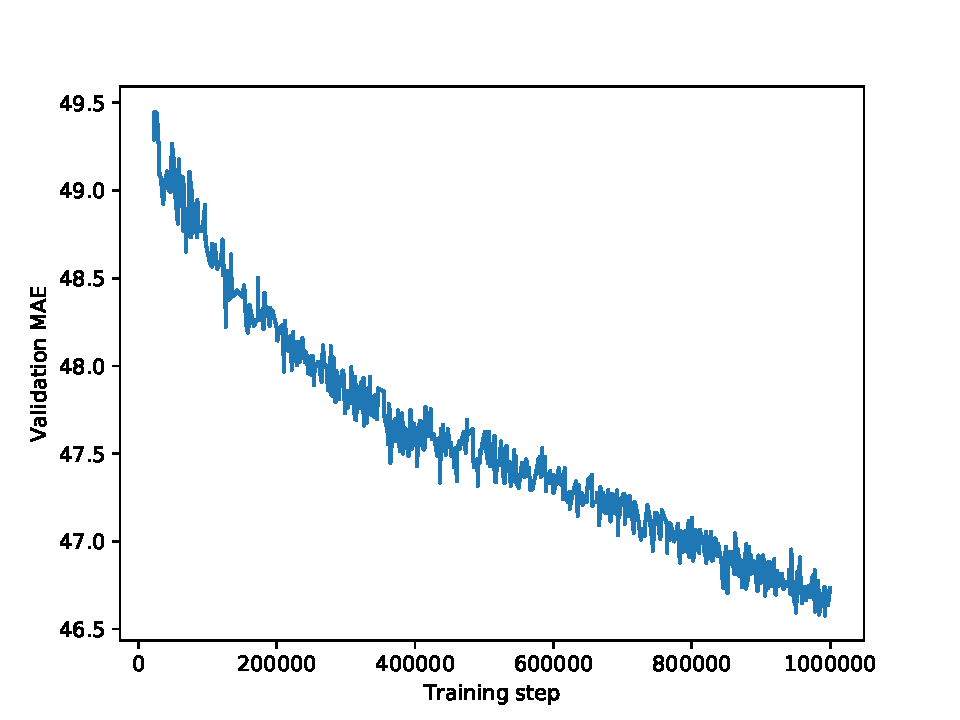
\includegraphics[width=0.5\textwidth]{image/loss.pdf}
  \caption{\label{fig:loss}Validation loss during training.}
\end{figure}

We experimented with other training schemes.
With teacher forcing, the decoder only receives ground truth sequences during training,
which might differ significantly from the autoregressively generated sequences
which it depends on for inference.
Therefore we tried training the model with free-running inputs.
We ran the model autoregressively to produce a sequence,
and used that sequence as the input to predict the truth sequence.
We mixed the training schedule with teacher forcing.
It was expected that the predictions would worsen in free-running mode,
but in the long run, the model should become more robust.
However that was not what we found.
Free-running training always worsened the model,
even when evaluated in teacher-forcing mode.

We also tried training with backpropagation through time (BPTT).
Since the outputs are continuous variables,
we can connect them to the inputs for the next step,
and the computation for all steps can be chained for backpropagation.
Training with BPTT is slow and expensive in memory usage,
but it was also ineffective.
As a result, we committed to teacher-forcing training.
We used a batch size of 32,
and the training speed was \textasciitilde{}7.2 iterations per second on a graphics card.

The validation loss continued to drop after over one million training steps,
as shown in Figure~\ref{fig:loss}.
However we decided to terminate the training process,
since each example has been seen a few thousand times.

\section{Results}\label{sec:results}

\begin{figure}
  \begin{subfigure}{0.5\textwidth}
    \centering
    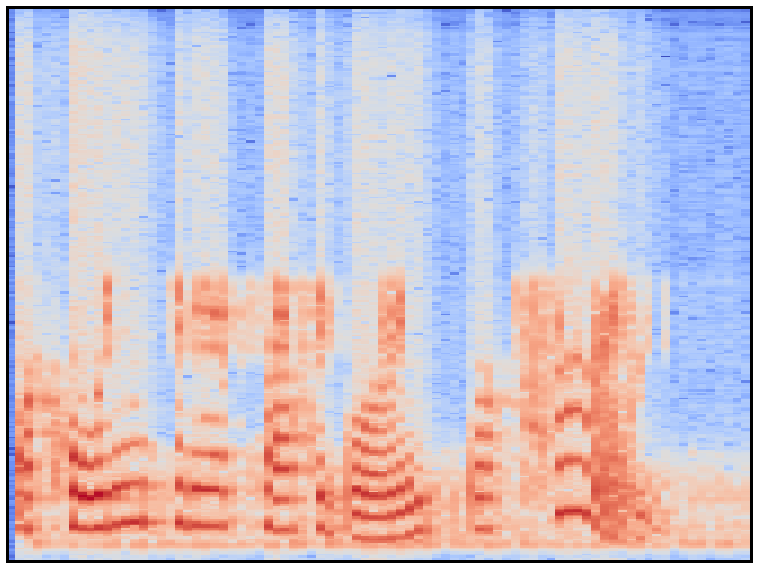
\includegraphics[width=0.9\textwidth]{image/forcing.pdf}
    \caption*{Teacher forcing}
  \end{subfigure}%
  \begin{subfigure}{0.5\textwidth}
    \centering
    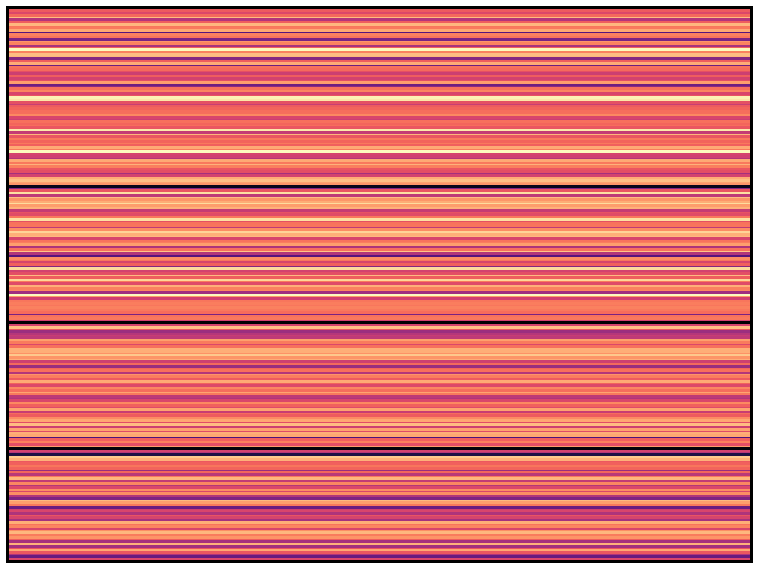
\includegraphics[width=0.9\textwidth]{image/autoreg.pdf}
    \caption*{Autoregressive}
  \end{subfigure}
  \caption{\label{fig:recons}Reconstructed spectrograms, cf.~\ref{fig:downsampled}.}
\end{figure}

In teacher-forcing mode, the model was able to reconstruct a spectrogram similar to the original.
The restored audio was intelligible but with a lower quality.
However when used autoregressively, the model failed to produce speech.
Figure~\ref{fig:recons} shows the results for an example in the validation data.

\begin{figure}
  \begin{subfigure}{0.5\textwidth}
    \centering
    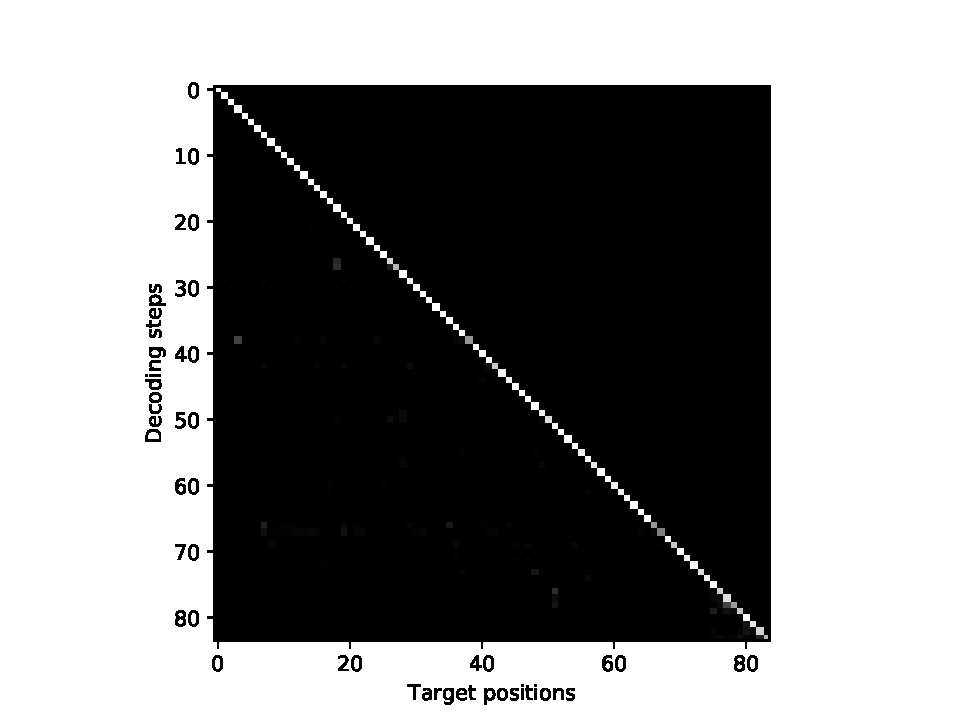
\includegraphics[width=\textwidth, trim={2cm 0 2cm 0}, clip]{image/attention_decoder_forcing.pdf}
    \caption*{Teacher forcing}
  \end{subfigure}%
  \begin{subfigure}{0.5\textwidth}
    \centering
    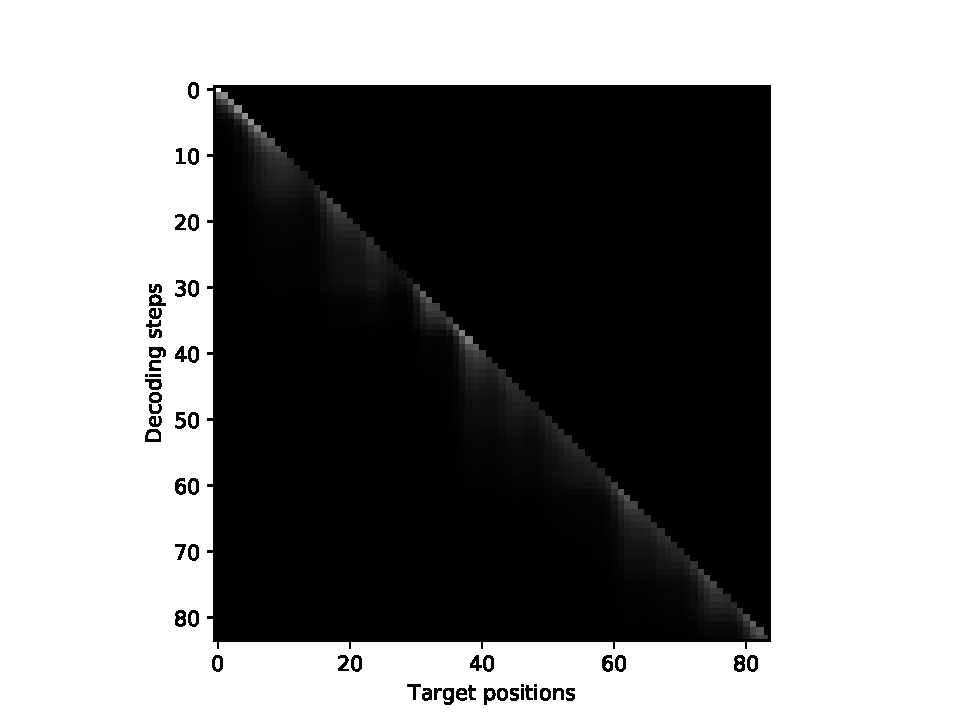
\includegraphics[width=\textwidth, trim={2cm 0 2cm 0}, clip]{image/attention_decoder_autoreg.pdf}
    \caption*{Autoregressive}
  \end{subfigure}
  \caption{\label{fig:att-decoder}Decoder self-attention alignment.}
\end{figure}

By inspecting the decoder attention alignment, as shown in Figure~\ref{fig:att-decoder},
we suspected that the cause of failure in autoregressive mode was that training in teacher-forcing mode
did not impose enough challenge to force the model to learn the mapping from the transcripts to the spectrograms.
The gradual nature of speech progression makes adjacent frames heavily correlated.
On top of that, since we used half-overlap for STFT,
the current spectrogram frame contains half of the information
in the next frame which the model was trained to predict.
The decoder alone may be able to produce a reconstruction with little training loss
when the ground-truth sequence was given as the input.
We attempted training schemes other than teacher forcing,
as discussed in Section~\ref{ssec:training},
which did not help to solve the problem.
Therefore we considered to increase the challenge by removing the frame overlap,
and used the Boxcar window for STFT instead of the Hanning window.
This however only lowered the quality of reconstruction during teacher-forcing mode,
and the model still failed in autoregressive mode.

\begin{figure}
  \begin{subfigure}{0.5\textwidth}
    \centering
    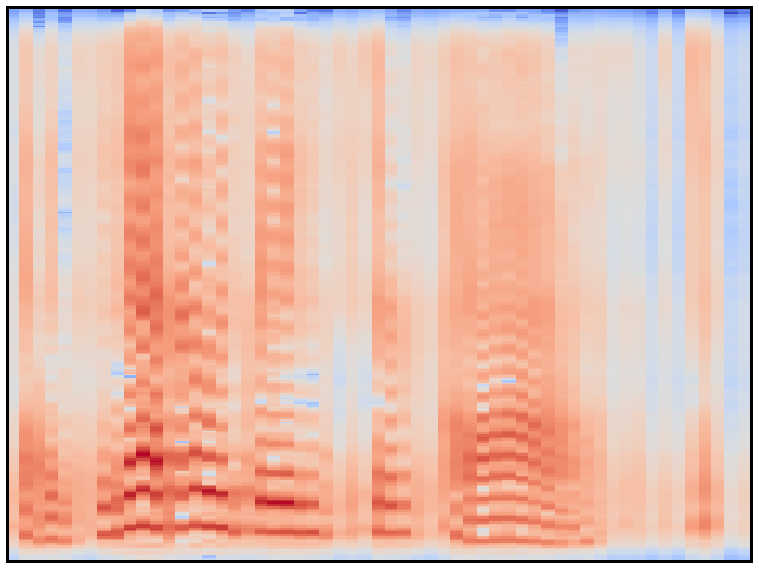
\includegraphics[width=0.9\textwidth]{image/magn_forcing.pdf}
    \caption*{Teacher forcing}
  \end{subfigure}%
  \begin{subfigure}{0.5\textwidth}
    \centering
    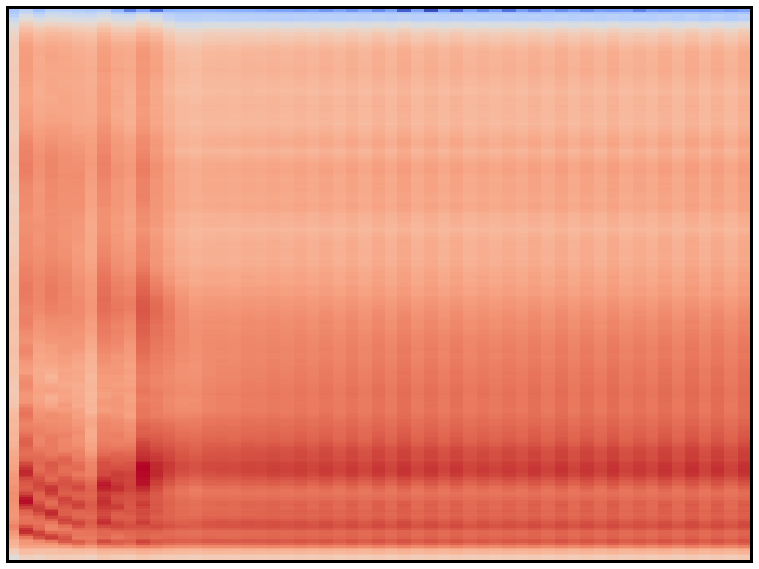
\includegraphics[width=0.9\textwidth]{image/magn_autoreg.pdf}
    \caption*{Autoregressive}
  \end{subfigure}
  \caption{\label{fig:recons-magn}Magnitude-only reconstruction, cf.~\ref{fig:recons}.}
\end{figure}

We considered the possibility that it was too difficult to learn
the reconstruction of the full complex-valued spectrograms.
Therefore we tried training the model only on the magnitude spectrograms.
As shown in Figure~\ref{fig:recons-magn},
this was indeed easier for the model to learn,
as the reconstruction was more detailed and closer to the original in Figure~\ref{fig:downsampled}.
However the model also failed to function in autoregressive mode.

The main challenge of training an encoder-decoder with attention was for the model the learn the alignment
between the two parts of the model.
In Tacotron, \textcite{wang2017tacotron} reported that
the attention tended to get stuck for multiple frames before moving forward,
and that either scheduled sampling \parencite{bengio2015scheduled}
or a bottleneck layer in the preprocessing network with a high dropout rate
was necessary for the model to learn a successful alignment.
On top of that, they found that predicting multiple frames at a time
helped to the model to learn a more stable alignment faster during training,
since it allowed the attention to move forward early.
In Tacotron 2, \textcite{shen2018natural} used location-sensitive attention
\parencite{chorowski2015attention} which had the additional feature
of cumulative attention weights from previous decoding steps
to encourage the alignment to move forward.
In Deep Voice 2, \textcite{arik2017deep2} reported that trimming the initial
silence in all audio clips was necessary was necessary for learning
the attention alignment.
In Deep Voice 3, \textcite{ping2017deep} enforced monotonic attention
\parencite{raffel2017online} to prevent the alignment from getting stuck.
In Char2Wav, \textcite{sotelo2017char2wav} used location-based attention
\parencite{graves2013generating} to hard-code location information into
the attention weights.
We had wished to avoid location-related constraints and allow the model
the freedom to learn the natural progression of speech by improving
the effectiveness of the attention mechanism.
However these strategies seem to be necessary in the TTS task.
Our model failed to learn the alignment between the encoder and the decoder,
as shown in Figure~\ref{fig:att-decoder}.

\begin{figure}
  \begin{subfigure}{0.5\textwidth}
    \centering
    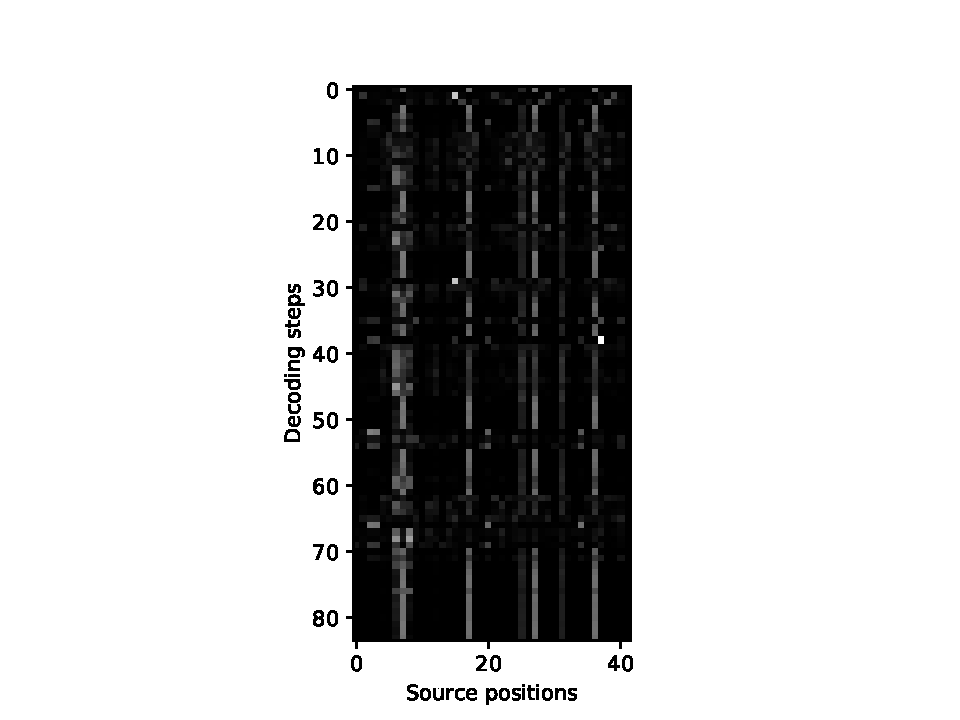
\includegraphics[width=\textwidth, trim={3cm 0 3cm 0}, clip]{image/attention_forcing.pdf}
    \caption*{Teacher forcing}
  \end{subfigure}%
  \begin{subfigure}{0.5\textwidth}
    \centering
    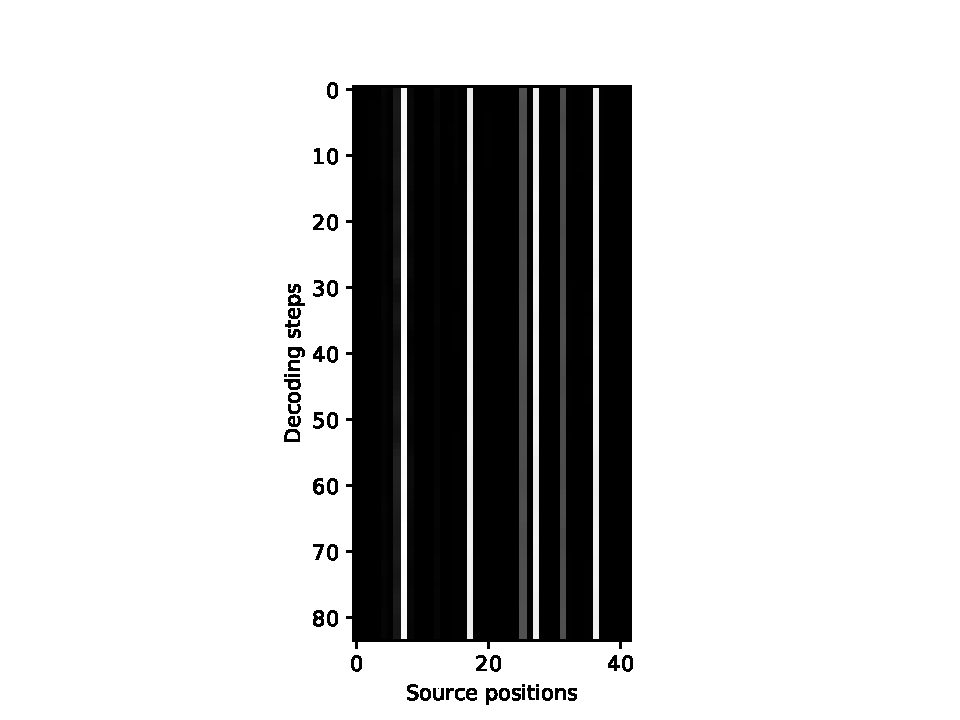
\includegraphics[width=\textwidth, trim={3cm 0 3cm 0}, clip]{image/attention_autoreg.pdf}
    \caption*{Autoregressive}
  \end{subfigure}
  \caption{\label{fig:att-decoder}Encoder-decoder attention alignment.}
\end{figure}

% attention_encoder.pdf

The architecture of our model was most similar to Tacotron,
except that we replaced the recurrent layers and CBHG networks with self-attention layers.
Despite the advantages of attention layers over convolutional and recurrent layers,
its modeling capacity remains a topic of investigation.
Recurrent networks have shown to be Turing complete \parencite{siegelmann1995computational}.
The design of self-attention layers still needs improvement in order to bridge the gap
\parencite{dehghani2018universal}.
Tacotron also used a CBHG post-processing network to convert mel spectrograms
to linear ones.
Since our model predicted linear spectrograms,
we only used an MLP after the decoder.
Although the mapping between linear scale and mel scale is simply a linear transformation,
the CBHG network helped to improve the quality of the outputs.
The mel scale magnifies information relevant to human speech,
so that the main encoder-decoder model may focus on learning the text-to-speech alignment,
while the post-processing network handles the details of the reconstruction.
In the future we would like to adopt the same approach.

\section{Conclusion}\label{sec:conclusion}

Our attempt at speech synthesis with complex-valued output
using the transformer architecture was not successful.
We analyzed the causes of failures and made suggestion for future research.
We underestimated the difficulties of the Task,
specifically in learning the attention alignment between the encoder and the decoder,
and in producing full complex-valued spectrograms.
As an afterthought, it would have been better to start with an existing model,
such as Tacotron, and gradually adapt changes to incorporate our goals.

\printbibliography[]
\end{document}
